\chapter*{LAMPIRAN} \addcontentsline{toc}{chapter}{LAMPIRAN}

\setcounter{\thechapter}{L}

\section{Data, Grafik dan Kode Program Percobaan Alat}
Adapun kode program, tabel data, grafik dan analisis hasil percobaan dapat dilihat pada Repository Github Berikut.
\begin{figure}[htbp]
    \centering
    
\includegraphics[width=0.4\textwidth]{images/qrcode_lampiran.png}
    \caption{QR Code Repository Github
    \url{https://github.com/Ajitot/KoefisienRestitusiIOTApp/}
    }
    \label{fig:qrcode_lampiran}
\end{figure}

\section{Dokumentasi Percobaan}
\subsection{Dokumentasi Video}

Dokumentasi video percobaan alat yang digunakan dalam penelitian ini dapat dilihat pada tautan berikut \url{https://www.youtube.com/watch?v=DF5Xv9Hjd88}.

\subsection{Dokumentasi Foto}
\begin{figure}[!htbp]
    \centering
    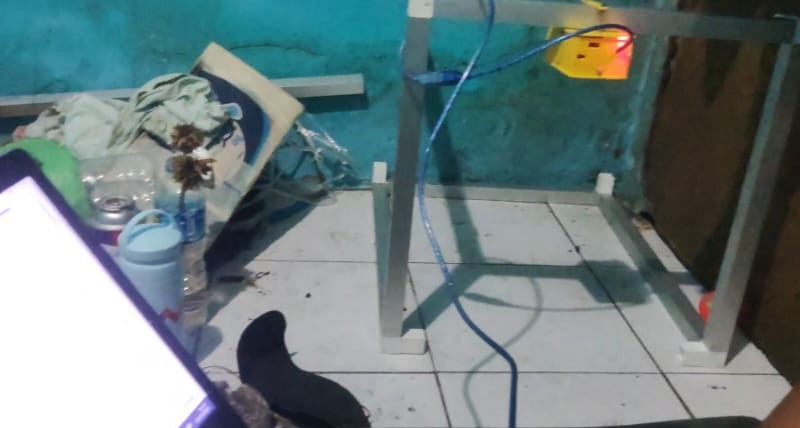
\includegraphics[width=0.5\linewidth]{images/Proses-Akuisisi-Data.jpeg}
    \caption{Proses pengambilan data}
    \citep{ajitot2024koefisien}
    \label{fig:pengambilan-data}
\end{figure}
\begin{figure}[!htbp]
    \centering
    \begin{subfigure}[b]{0.45\linewidth}
        \centering
        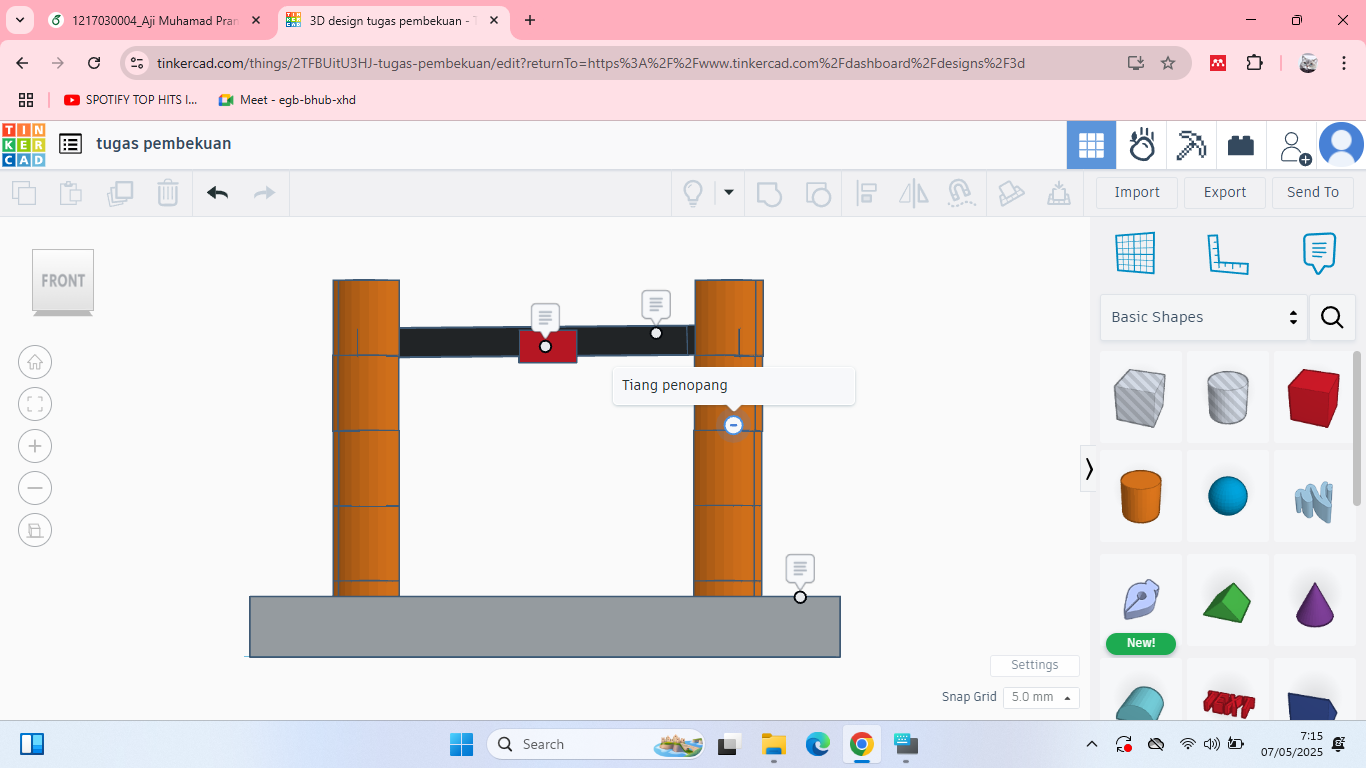
\includegraphics[width=\linewidth]{images/Screenshot (2).png}
        \caption{Ilustrasi alat 1}
        \label{fig:ilustrasi-alat-1}
    \end{subfigure}
    \hfill
    \begin{subfigure}[b]{0.45\linewidth}
        \centering
        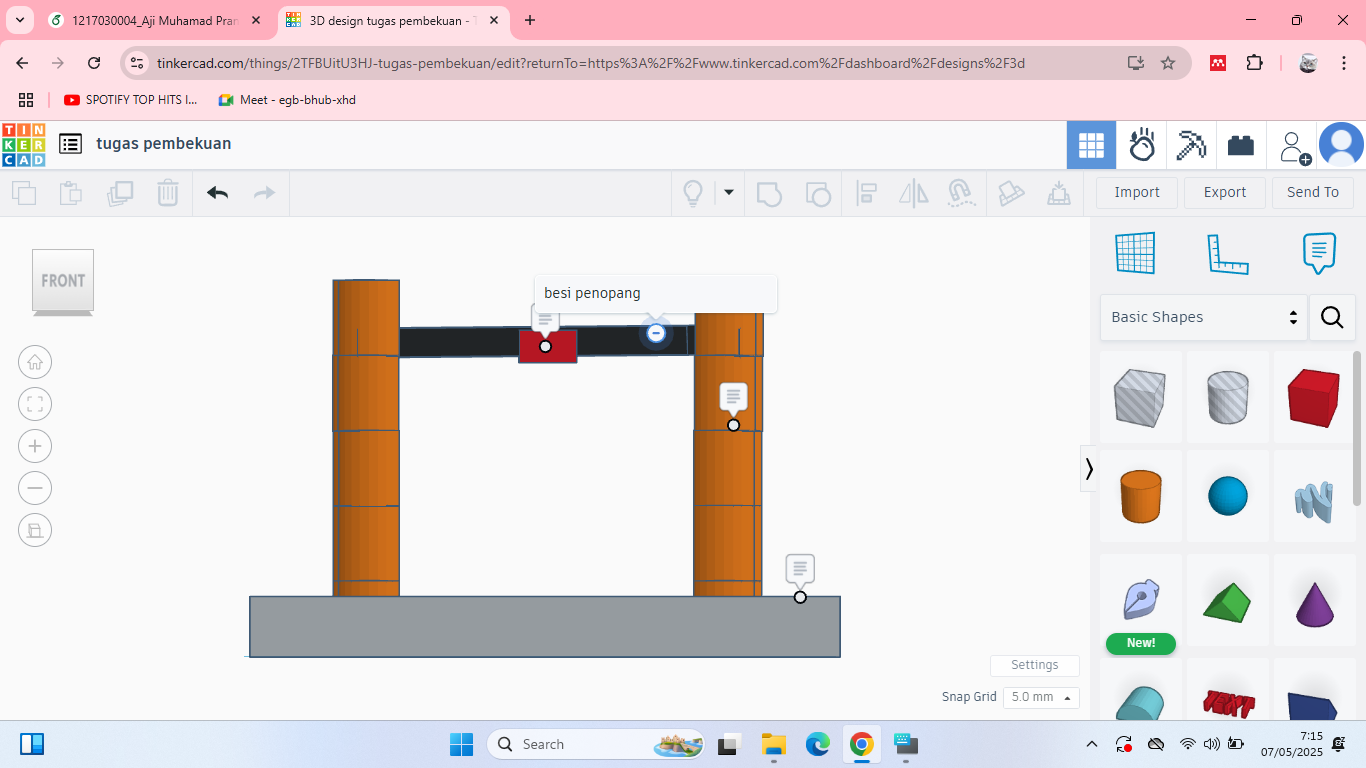
\includegraphics[width=\linewidth]{images/Screenshot (3).png}
        \caption{Ilustrasi alat 2}
        \label{fig:ilustrasi-alat-2}
    \end{subfigure}
    \vskip\baselineskip
    \begin{subfigure}[b]{0.45\linewidth}
        \centering
        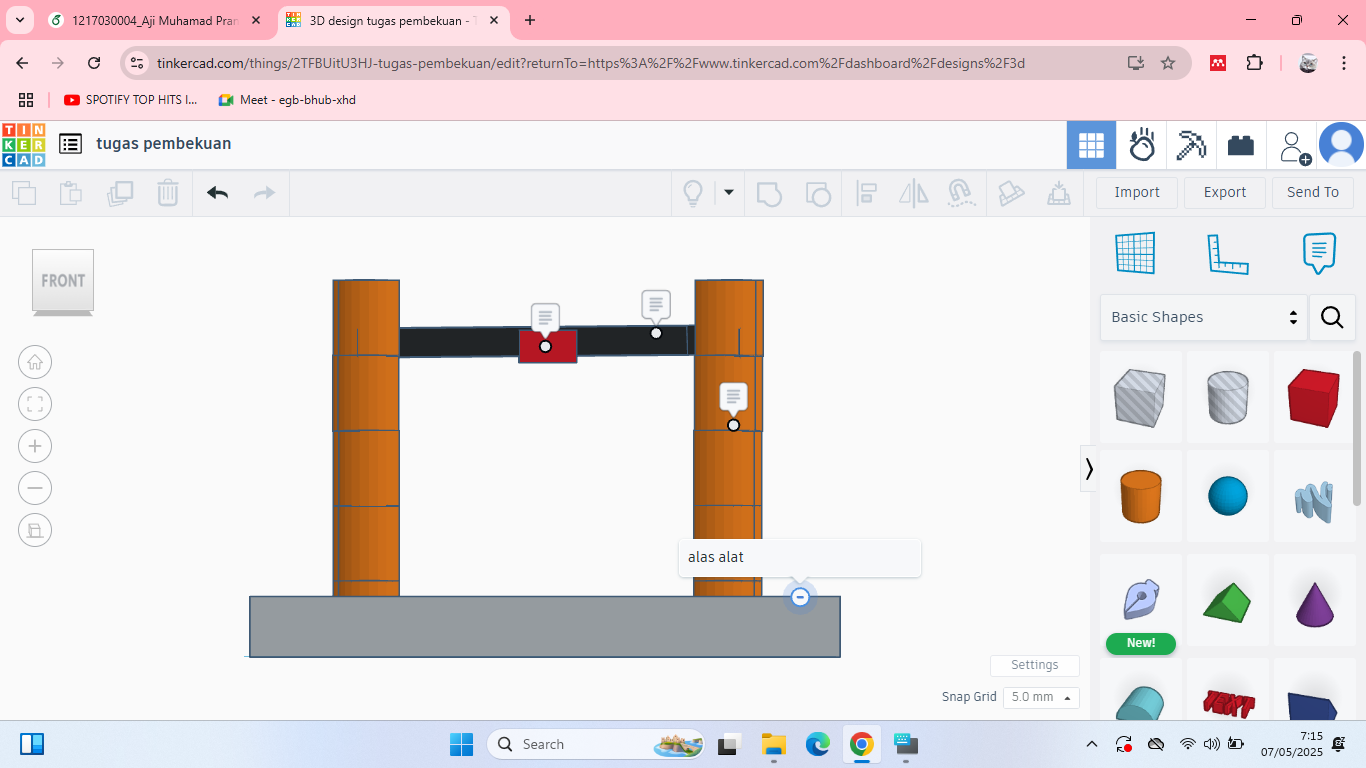
\includegraphics[width=\linewidth]{images/Screenshot (4).png}
        \caption{Ilustrasi alat (tampak depan)}
        \label{fig:ilustrasi-alat-depan}
    \end{subfigure}
    \hfill
    \begin{subfigure}[b]{0.45\linewidth}
        \centering
        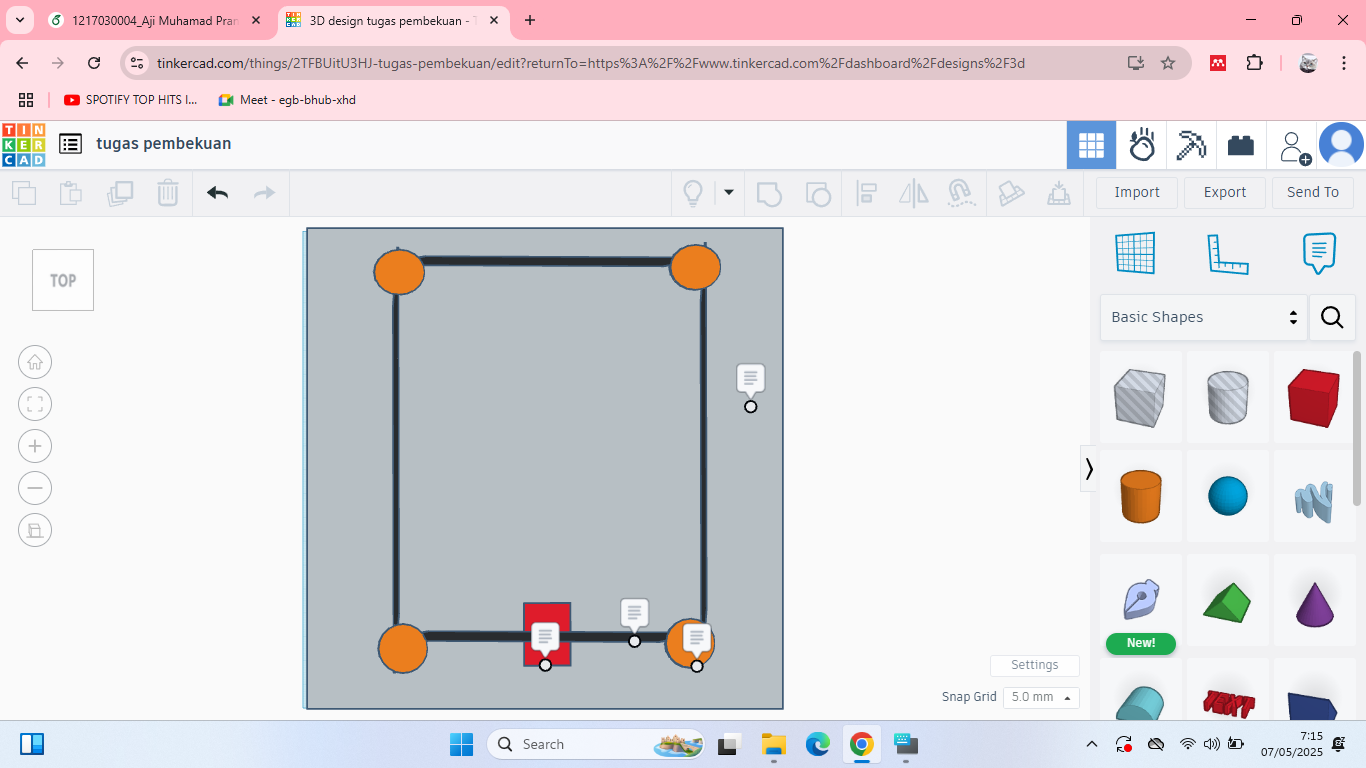
\includegraphics[width=\linewidth]{images/Screenshot (5).png}
        \caption{Ilustrasi alat (tampak atas)}
        \label{fig:ilustrasi-alat-atas}
    \end{subfigure}
    \caption{Ilustrasi alat dari berbagai sudut}
    \label{fig:ilustrasi-alat-semua}
\end{figure}

\newpage

\section{Penurunan Persamaan Koefisien Restitusi}
\begin{figure}[htbp]
    \centering
    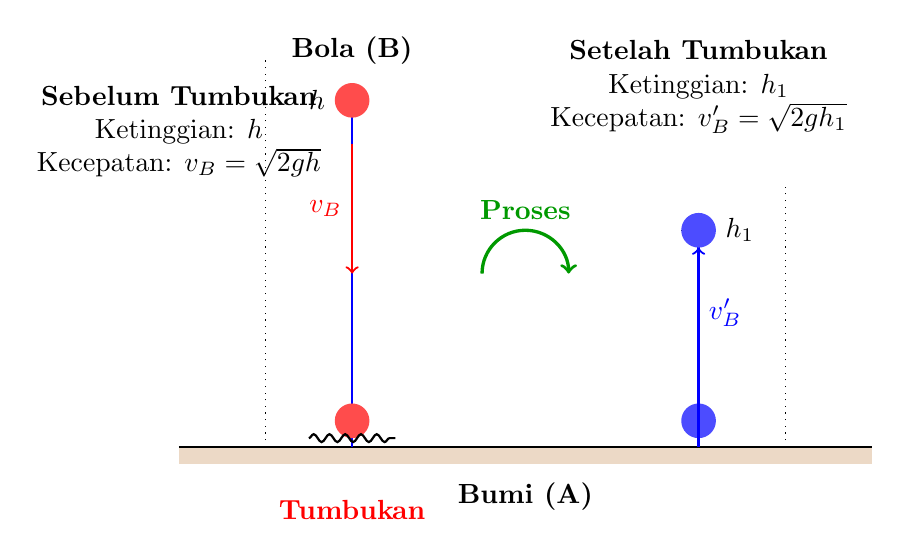
\begin{tikzpicture}[scale=1.1]
        % Ground/Earth Representation
        \fill[brown!30] (-4,-0.2) rectangle (4,0);
        \draw[thick] (-4,0) -- (4,0);
        \node[below] at (0,-0.3) {\textbf{Bumi (A)}};

        % Initial Position - Ball At Height H
        \draw[blue, thick] (-2,0) -- (-2,4);
        \draw[dashed] (-2.2,4) -- (-1.8,4);
        \node[left] at (-2.2,4) {$h$};

        % Ball At Initial Height
        \fill[red!70] (-2,4) circle (0.2);
        \node[above] at (-2,4.3) {\textbf{Bola (B)}};

        % Velocity Arrow Before Collision
        \draw[->, thick, red] (-2,3.5) -- (-2,2) node[midway, left] {$v_B$};

        % Ball Just Before Collision
        \fill[red!70] (-2,0.3) circle (0.2);

        % Collision Point Indicator With Wavy Line Instead Of Zigzag
        \draw[thick, decorate, decoration={snake, amplitude=0.5mm, segment length=2mm}] (-2.5,0.1) -- (-1.5,0.1);
        \node[below] at (-2,-0.5) {\textcolor{red}{\textbf{Tumbukan}}};

        % Ball After Collision (Bouncing Up)
        \fill[blue!70] (2,0.3) circle (0.2);

        % Velocity Arrow After Collision
        \draw[->, thick, blue] (2,0.8) -- (2,2.3) node[midway, right] {$v'_B$};

        % Final Position - Ball At Height H₁
        \draw[blue, thick] (2,0) -- (2,2.5);
        \draw[dashed] (1.8,2.5) -- (2.2,2.5);
        \node[right] at (2.2,2.5) {$h_1$};

        % Ball At Final Height
        \fill[blue!70] (2,2.5) circle (0.2);

        % Labels For Phases
        \node[above, align=center] at (-4,3) {\textbf{Sebelum Tumbukan}\\Ketinggian: $h$\\Kecepatan: $v_B = \sqrt{2gh}$};
        \node[above, align=center] at (2,3.5) {\textbf{Setelah Tumbukan}\\Ketinggian: $h_1$\\Kecepatan: $v'_B = \sqrt{2gh_1}$};

        % Arrow Showing The Process
        \draw[->, very thick, green!60!black] (-0.5,2) arc (180:0:0.5) node[midway, above] {\textbf{Proses}};

        % Reference Line For Heights
        \draw[dotted] (-3,0) -- (-3,4.5);
        \draw[dotted] (3,0) -- (3,3);
    \end{tikzpicture}
\end{figure}

\newpage
\textbf{Keterangan:}
\begin{itemize}
    \item A = Bumi
    \item B = Bola
    \item $h$ = Ketinggian Awal Bola
    \item $h_1$ = Ketinggian Akhir Bola
    \item $v_B$ = Kecepatan Sebelum Tumbukan Bola
    \item $v'_B$ = Kecepatan Setelah Tumbukan Bola
\end{itemize}
\subsection*{Hukum Kekekalan Momentum}
\begin{align}
    p_A + p_B &= p'_A + p'_B \\
    m_A v_A + m_B v_B &= m_A v'_A + m_B v'_B \\
    m_A v_A - m_A v'_A &= m_B v'_B - m_B v_B \\
    m_A (v_A - v'_A) &= m_B (v'_B - v_B) \quad \text{...(1)}
\end{align}

\subsection*{Hukum Kekekalan Energi Kinetik}
\begin{align}
    EK_A + EK_B &= EK'_A + EK'_B \\
    \frac{1}{2} m_A v_A^2 + \frac{1}{2} m_B v_B^2 &= \frac{1}{2} m_A {v'_A}^2 + \frac{1}{2} m_B {v'_B}^2 \\
    m_A v_A^2 - m_A {v'_A}^2 &= m_B {v'_B}^2 - m_B v_B^2 \\
    m_A (v_A^2 - {v'_A}^2) &= m_B ({v'_B}^2 - v_B^2) \quad \text{...(2)}
\end{align}

Membagi persamaan (2) dengan persamaan (1):
\begin{align}
    \frac{m_A (v_A^2 - {v'_A}^2)}{m_A (v_A - v'_A)} &= \frac{m_B ({v'_B}^2 - v_B^2)}{m_B (v'_B - v_B)}
\end{align}

Karena \( m_A \) dan \( m_B \) ada di pembilang dan penyebut, kita dapat menyederhanakan:
\begin{equation}
    \frac{(v_A^2 - {v'_A}^2)}{(v_A - v'_A)} = \frac{({v'_B}^2 - v_B^2)}{(v'_B - v_B)}
\end{equation}

Gunakan identitas pemfaktoran untuk selisih kuadrat:
\begin{gather}
    v_A^2 - {v'_A}^2 = (v_A - v'_A)(v_A + v'_A) \\
    {v'_B}^2 - v_B^2 = (v'_B - v_B)(v'_B + v_B)
\end{gather}

Masukkan ke dalam persamaan:
\begin{equation}
    \frac{(v_A - v'_A)(v_A + v'_A)}{(v_A - v'_A)} = \frac{(v'_B - v_B)(v'_B + v_B)}{(v'_B - v_B)}
\end{equation}

Karena \( (v_A - v'_A) \) dan \( (v'_B - v_B) \) ada di pembilang dan penyebut, kita bisa menyederhanakan:
\begin{align}
    v_A + v'_A &= v'_B + v_B \\
    v_A - v_B &= v'_B - v'_A \\
    -(v_B - v_A) &= v'_B - v'_A \\
    1 &= \frac{v'_B - v'_A}{v_B - v_A}
\end{align}
Angka "1" di atas menunjukkan nilai koefisien restitusi untuk tumbukan lenting 
sempurna, sehingga secara umum persamaan koefisien restitusi untuk tumbukan adalah sebagai berikut.
\begin{equation}
        e = \frac{v'_B - v'_A}{v_B - v_A}
\end{equation}

Pada saat bola jatuh bebas ke bawah berlaku hukum kekekalan energi sehingga kita 
dapat menentukan kecepatan benda sesaat sebelum bertumbukan dengan lantai 
seperti berikut. 
\begin{align}
    E_P &= E_K \\
    mgh &= \frac{1}{2} mv^2 \\
    gh &= \frac{1}{2} v^2 \\
    v^2 &= 2gh \\
    v &= \sqrt{2gh}
\end{align}

Dengan menggunakan cara yang sama seperti di atas, maka kita dapat menentukan 
hubungan antara kecepatan di dasar dengan ketinggian seperti berikut:
\begin{gather}
    v_B = \sqrt{2gh} \\
    v'_B = \sqrt{2gh_1}
\end{gather}

Untuk pemantulan pertama kita dapat menentukan koefisien restitusi yakni:
\begin{equation}
        e = \frac{v'_B - v'_A}{v_B - v_A}
\end{equation}

$ v'_A = v_A = 0 $ (Diam Terhadap Bola).
($v$ bernilai negatif karena arahnya ke bawah)
\begin{align}
    e &= \frac{v_1}{v} \\
    e &= \sqrt{\frac{2gh_1}{2gh}} \\
    e &= \sqrt{\frac{h_1}{h}} 
\end{align}

